\documentclass[11pt,a4paper]{article}
\usepackage[utf8]{inputenc}
\usepackage{amsmath}
\usepackage{amsfonts}
\usepackage{amssymb}
\usepackage{tikz}
\author{Mikkel Riber Bojsen - s093255}
\begin{document}
\section{$\mathcal{NP}$-completeness}

To prove $\mathcal{NP}$-completeness, we look at the problem \textsc{PartitionByPairs} (PBP). 

\subsection{Transformation}
Given an instance $X$ of PBP, we do the following transformation ($T(X)$). We calculate the value $B = \frac{\sum_{i=1}^{2n} s_i}{2}$. For each pair $(s_{2i-1}, s_{2i})$ in $S$,  where $i \in \lbrace 1,\dots, n \rbrace $, we construct a graph as show in Fig.~\ref{fig:transform1}, where the labels are the weights of the corresponding edge. 

\begin{figure}[!htb]
\centering
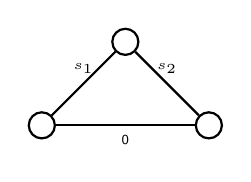
\begin{tikzpicture}[auto,node distance=1.5cm,
  thick,main node/.style={circle,draw,font=\sffamily\tiny\bfseries}]

  \node[main node] (1) {};
  \node[main node] (2) [above right of=1] {};
  \node[main node] (3) [below right of=2] {};
 % \node[main node] (4) [right of=3] {4};

  \path[every node/.style={font=\sffamily\tiny}]
    (1) edge node [above] {$s_1$} (2)
    	edge [right] node [below] {0} (3)
    (2) edge node [above] {$s_2$} (3);
    %	edge [bend left] node {0} (4)
   % (3) edge node {$s_2$} (4);

\end{tikzpicture}
\caption{Transformation of a single pair}
\label{fig:transform1}
\end{figure}

We order the set of edges, so the mirror of the edge with weight $s_{2i-1}$ is $s_{2i}$ and the mirror of an edge with weight 0 is an edge with weight 0 (if there is an odd number of pairs, the middle edge will be a zero that mirrors into itself). For multiple pairs, we chain multiple graphs together as shown in Fig.~\ref{fig:transform2}. 
\begin{figure}[htb]
\resizebox{\linewidth}{!}{
\centering
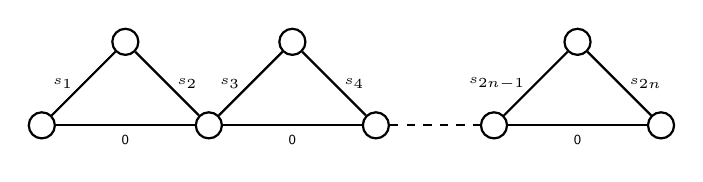
\begin{tikzpicture}[auto,node distance=1.5cm,
  thick,main node/.style={circle,draw,font=\sffamily\small\bfseries}]

  \node[main node] (1) {};
  \node[main node] (2) [above right of=1] {};
  \node[main node] (3) [below right of=2] {};
  \node[main node] (4) [above right of=3] {};
  \node[main node] (5) [below right of=4] {};
  \node[main node] (6) [right of=5] {};
  \node[main node] (7) [above right of=6] {};
  \node[main node] (8) [below right of=7] {};


  \path[every node/.style={font=\sffamily\tiny}]
    (1) edge node [left] {$s_1$} (2)
    	edge [right] node [below] {0} (3)
    (2) edge node [right] {$s_2$} (3)
    
     (3) edge node [left] {$s_3$} (4)
        	edge [right] node [below] {0} (5)
        (4) edge node [right] {$s_4$} (5)
    	
     (6) edge node [left] {$s_{2n-1}$} (7)
        	edge [right] node [below] {0} (8)
        (7) edge node [right] {$s_{2n}$} (8)
        
        ;
             
   \draw[style=dashed, ] (5) -- (6);
\end{tikzpicture}}
\caption{Transformation of several pairs}
\label{fig:transform2}
\end{figure}

For example, the set $S=\lbrace 1,2,3,4,5,6 \rbrace$ is transformed into a list of weights $W=[1,3,5,0,0,0,6,4,2]$, where the weight of edge $i$ is the $i$'th element in $W$.
\noindent
Using this graph and the calculated value $B$ we can query MFMST to answer PBP.

\subsection{Proof}

We do our transformation in polynomial time. The calculation of $B$ is done in $O(n)$. For each pair, we construct a constant number of nodes and edges, so the graph can be created in $O(n)$, this means our transformation can be done in $O(n)$.

If the answer to the original problem instance $X$ is YES, it means that a partition where we pick one from each pair equals $B$. It is possible to pick a spanning tree where we pick one from each pair as shown in Fig~\ref{fig:transform3}. As the answer to the original problem was YES, and we can pick a spanning tree that uses an edge from each pair, the answer must also be YES to $T(X)$.

\begin{figure}[htb]
\resizebox{\linewidth}{!}{
\centering
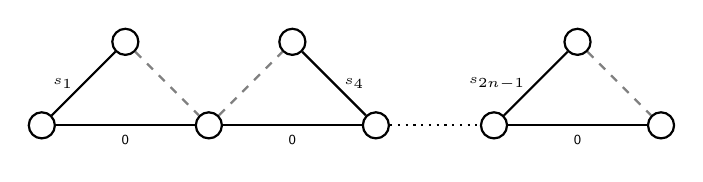
\begin{tikzpicture}[auto,node distance=1.5cm,
  thick,main node/.style={circle,draw,font=\sffamily\small\bfseries}]

  \node[main node] (1) {};
  \node[main node] (2) [above right of=1] {};
  \node[main node] (3) [below right of=2] {};
  \node[main node] (4) [above right of=3] {};
  \node[main node] (5) [below right of=4] {};
  \node[main node] (6) [right of=5] {};
  \node[main node] (7) [above right of=6] {};
  \node[main node] (8) [below right of=7] {};


  \path[every node/.style={font=\sffamily\tiny}]
    (1) edge node [left] {$s_1$} (2)
    	edge [right] node [below] {0} (3)
   % (2) edge node [right] {$s_2$} (3)
    
     (3) % edge node [left] {$s_3$} (4)
        	edge [right] node [below] {0} (5)
        (4) edge node [right] {$s_4$} (5)
    	
     (6) edge node [left] {$s_{2n-1}$} (7)
        	edge [right] node [below] {0} (8)
   %     (7) edge node [right] {$s_{2n}$} (8)
        
        ;
             
   \draw[style=dotted, ] (5) -- (6);
    \draw[color=gray, dashed] (2) -- (3);
        \draw[color=gray, dashed] (3) -- (4);
            \draw[color=gray, dashed] (7) -- (8);
\end{tikzpicture}}
\caption{A spanning tree}
\label{fig:transform3}
\end{figure}

We now assume the answer to the original problem is NO. In this case, we know that it is not possible to pick one edge from each pair in the transformation and get a value that is exactly $B$. 

Any spanning tree must pick at least one from each pair, but can pick two (ignoring the $0$-edge) and all edge weights are non-negative. 

If we pick more than one edge from a pair, we increase both the weight of the spanning tree and the mirror, as the two edges we pick are mirrors of each other, and therefore will be in both sums.

In summary, this means that if the original answer is NO, we cannot pick a spanning tree using one from each pair, where the maximum value of the tree and the mirror is exactly $B$. As we need to pick at least one from each pair to have a spanning tree, and picking more than one, always increases both values, we cannot get a spanning tree that will make MFMST answer NO.

As our transformation runs in polynomial time, the original problem is $\mathcal{NP}-complete$, our transformation preserves the original answer and MFMST is in $\mathcal{NP}$, we can conclude that MFMST is $\mathcal{NP}-complete$.


\section{Optimization Algorithm Description}

\subsection{General algorithm}
Our algorithm does an exhaustive search of spanning trees, while storing the tree ($T$) scoring lowest in the equation

$$
\max \left\{ \sum_{e_i \in T} w(e_i), \sum_{e_i \in T} w(e_{m+1-i}) \right\}
$$

In the algorithm, we treat the graph as being a weighed, directed multigraph, to allow multiple edges between nodes.
The spanning trees are found by doing so-called cuts and contracts.  This creates a recursive computation as follows:

\vspace{0.5cm}
\noindent
If no edge remain, stop the calculation. Otherwise, pick an edge and:

\begin{enumerate}
\item Create a copy of the graph, where the end-points of this edge is merged into one point and any edges between them are removed. Store which edge was contracted.

\begin{itemize}
\item Use depth first search from an end-point of the contracted edge through the set of contracted edges, to make sure no cycle was created. 

\item If a cycle is created, stop the calculation of this path, otherwise, calculate all spanning trees on the copy.
\end{itemize}

\item Create a copy of the graph where the edge is removed.
\begin{itemize}
\item Do a depth first search from one end-point of the removed edge.

\item If the other end-point is reached, calculate all spanning trees on the copy.

\item If the other end-point it not reached, the graph has been disconnected, stop the calculation of this path.
\end{itemize}
\end{enumerate} 

Every leaf of this computation tree contains a unique spanning tree. It can be found by collecting all stored edges from leaf to root.

\subsection{Computation tree}

An example of such a computation tree can be seen in \Cref{fig:comptree}, where all possible cuts and contracts that can be made are shown for the example graph from \Cref{fig:example}. Every node corresponds to a copy of the original graph, where edges have been cut or contracted, according to the path to the root. The lines/nodes are grayed out when a cycle has been created (during a \texttt{contract}), or the graph has been split into multiple connected components (during a \texttt{cut}). Finally one can see that three spanning trees are found, each one marked with a blue leaf node.

\begin{figure}[H]
\resizebox{\linewidth}{!}{
\centering
\begin{tikzpicture}[auto,node distance=1.5cm,font=\sffamily\tiny,
  thick,main node/.style={circle,draw,font=\sffamily\tiny},
  edge label/.style={midway,above,sloped,font=\sffamily\tiny}]

  \node[main node] (1) {1};
  \node[node distance=1.05cm] (1a) [left of=1] {};
  \node[node distance=1.05cm] (1b) [right of=1] {};
  \node[main node] (2) [below left of=1a] {2};
  \node[main node] (3) [below right of=1b] {3};
  
  \node[main node,blue] (4) [below left of=2] {4};
  \node[main node] (5) [below right of=2] {5};
  \node[main node] (6) [below left of=3] {6};
  \node[main node,opacity=0.4] (7) [below right of=3] {7};
  
  \node[main node,opacity=0.4] (8) [below left=0.8cm and 0.5cm of 4] {8};
  \node[main node,opacity=0.4] (9) [below right=0.8cm and 0.5cm of 4] {9};
  \node[main node,blue] (10) [below left=0.8cm and 0.5cm of 5] {10};
  \node[main node,opacity=0.4] (11) [below right=0.8cm and 0.5cm of 5] {};
  \node[main node,blue] (12) [below left=0.8cm and 0.5cm of 6] {};
  \node[main node,opacity=0.4] (13) [below right=0.8cm and 0.5cm of 6] {};
  \node[main node,opacity=0.4] (14) [below left=0.8cm and 0.5cm of 7] {};
  \node[main node,opacity=0.4] (15) [below right=0.8cm and 0.5cm of 7] {};
  
  \draw (1) -- (2) node[edge label] {contract};
  \draw (1) -- (3) node[edge label] {cut};
  
  \draw (2) -- (4) node[edge label] {contract};
  \draw (2) -- (5) node[edge label] {cut};
  \draw (3) -- (6) node[edge label] {contract};
  \draw[dashed,opacity=0.4] (3) -- (7) node[edge label] {cut};
  
  \draw[dashed,opacity=0.4] (4) -- (8) node[edge label]{contract};
  \draw[dashed,opacity=0.4] (4) -- (9) node[edge label] {cut};
  \draw (5) -- (10) node[edge label] {contract};
  \draw[dashed,opacity=0.4] (5) -- (11) node[edge label] {cut};
  \draw (6) -- (12) node[edge label] {contract};
  \draw[dashed,opacity=0.4] (6) -- (13) node[edge label] {cut};
  \draw[dashed,opacity=0.4] (7) -- (14) node[edge label] {contract};
  \draw[dashed,opacity=0.4] (7) -- (15) node[edge label] {cut};
 
 
  \node[font=\small] (L1) [below right=0.1cm and 4.5cm of 1] {$e_1$};
  \node[font=\small] (L2) [below=0.55cm of L1] {$e_2$};
  \node[font=\small] (L3) [below=0.55cm of L2] {$e_3$};

  \node[] (La1) [left=9cm of L1] {};
  \node[] (La2) [left=9cm of L2] {};
  \node[] (La3) [left=9cm of L3] {};
  
  \draw[dashed, thin, opacity=0.1] (L1) -- (La1);
  \draw[dashed, thin, opacity=0.1] (L2) -- (La2);
  \draw[dashed, thin, opacity=0.1] (L3) -- (La3);
\end{tikzpicture}}
\caption{Computation tree for the graph \Cref{fig:example} in order to find all the spanning trees. These have been marked with a blue nodes.}
\label{fig:comptree}
\end{figure}


\subsection{Tricks}
Since all edges have positive weights, we can maintain the current ``value'' of the calculation that has been created, i.e. the edges that have already been picked. If we maintain a best found solution, we can stop finding more trees once we reach this value, thereby hopefully cutting of branches from the computation tree.

To increase the number of branches we can cut off, we can try to guess a good edge to contract at every step, using one of two heuristics:

\begin{enumerate}
\item The edge $e_i$ with the lowest score of $\max\left\{w(e_i),w(e_{m+1-i})\right\}$  (maximum of edge/mirror)

\item The edge $e_i$ with the lowest score of $w(e_i)+w(e_{m+1-i})$ (sum of edge/mirror)
\end{enumerate}

If we sort all edges based on one of these heuristics, we will automatically try the ``best'' possibilities first. This can be done using any sorting algorithm, we have chosen \textsc{QuickSort}.

\section{Correctness}
To prove correctness of our algorithm, we need to show that we potentially search all spanning trees, and that the paths in the computation we decide not to follow, cannot contain a tree that is better suited than what we already have.

\subsection{Finding All Spanning Trees}

If we disregard the part where we cut of a path early, we first need to prove that we can search all spanning trees.

\noindent
Assume a spanning tree $T'$ exists which we did not check.

\begin{itemize}
\item If we did not find this tree, there is no leaf in our computation tree that corresponds to $T'$.

\item If $T'$ contains $e_1$, then we can move down the left edge of the root of the computation tree (contract). If $e_1$ is not in $T'$ we take the right edge from the root (cut).

\item This can be done for all edges, except those that would disconnect the graph if removed, or if using the edge creates a cycle in our current tree.

\item If $e_i$ is not in $T'$, but it would disconnect the graph, we do not have a leaf corresponding to $T'$.
\begin{itemize}
\item As $e_i$ would disconnect the graph, $T'$ cannot be a spanning tree.
\end{itemize}

\item If $e_j$ is in $T'$, but using it would create a cycle, we do not have a leaf that corresponds to $T'$.

\begin{itemize}
\item As $e_j$ would create a cycle in the tree being built, $T'$ cannot be a tree, and thus not a spanning tree.
\end{itemize}
\end{itemize}

The same argumentation works with any ordering of the edges in the algorithm.

\subsection{Correctness of Early Search Termination}
As we only have positive edge weights, we can always assume that an ongoing search for a tree, only increases in total weight. This means that once we reach our current best weight, it is impossible for any tree generated by the current search further down our computation tree to yield a better tree.

\subsection{Summary}
In summary, our algorithm is correct, as we potentially search all spanning trees of the graph and we only terminate a search if it impossible for the result to be better than what we already have.

\section{Running time}
If the input graph has $n$ nodes and $m$ edges, we have the following running times.

\begin{itemize}
\item We can calculate all the heuristic values for edges in $O(m)$

\item We can sort the edges by their heuristic value in expected $O(m\cdot \log m)$.

\item For every inner node in the computation tree we do the following:
\begin{itemize}
\item Perform a depth-first-search to see if an edge added to the contracted set, creates a loop. This can be done in $O(n+m)$.

\item Perform a depth-first-search to see if removing an edge splits the current graph in two components. This can be done in $O(m+n)$.
\end{itemize}

\item The computation tree is binary, and every leaf in the tree corresponds to a spanning tree. Cayleys formula states that a complete graph has $O(n^{n-2})$ spanning trees.

\item The path from a leaf to the root of the tree is at most $m$.

\item The computational tree has in the worst case, at most $O(m\cdot n^{n-2})$ nodes.
\end{itemize}

Summing this up, we get a running time of $O((m+n)\cdot m\cdot n^{n-2})$, as we perform two depth-first-searches for every inner node in the computation tree.
\end{document}